\section{Experimental Evaluation} \label{sec:extension_experiments}

\subsection{Kd-tree versus quadtree performance} \label{sec:comparison}
To compare the quadtree and kd-tree partition strategies, we analyze their performance across several stages: constructing the spatial data structure to define the partition cells based on the sample, the cost of partitioning, populating the cells with the full datasets, and the overall time required to complete each phase of the overlay operation using each partitioning approach. We use the MainUS and GADM datasets, as described in Table \ref{tab:datasets}.

 \begin{figure}
    \centering
    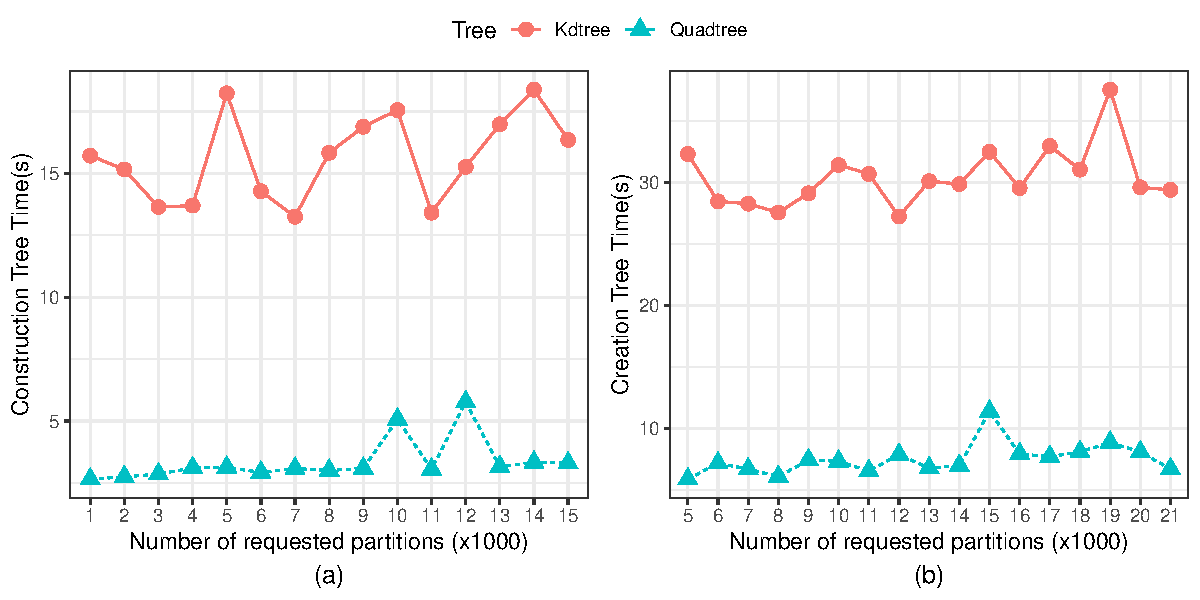
\includegraphics[width=\textwidth]{chapterExtension/K/K_Creation}
    \caption{Construction time for the spatial data structure in the (a) MainUS and (b) GADM datasets.}\label{fig:k_creation_us}
 \end{figure}

Figure \ref{fig:k_creation_us} illustrates the construction time for sampling the input layers and generating partitioning cells with varying numbers of divisions. The kd-tree requires more time, primarily due to the sorting involved at each split to organize the data and locate the midpoint. On average, the quadtree takes only 23.13\% of the time needed to create the kd-tree (21.55\% for MainUS and 24.72\% for GADM). However, kd-tree creation accounts for only 5.86\% of the total time required for complete DCEL construction (6.88\% for MainUS and 4.87\% for GADM).

 \begin{figure}
    \centering
    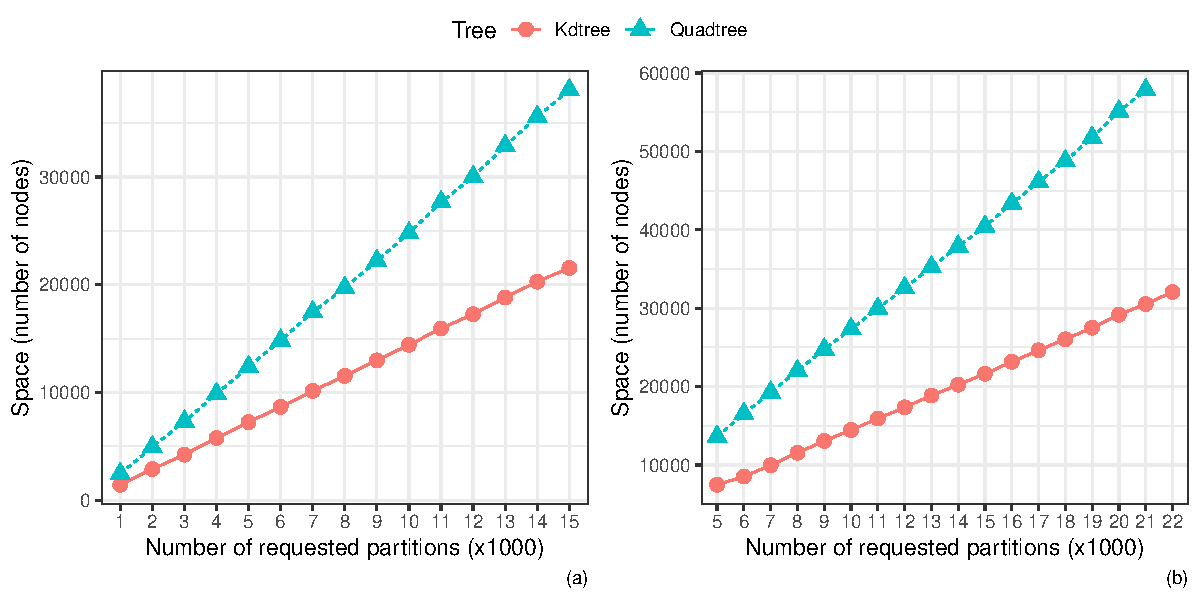
\includegraphics[width=\textwidth]{chapterExtension/K/K_Space} 
    \caption{Number of cells created by each spatial data structure in the (a) MainUS and (b) GADM datasets.} \label{fig:k_space_us}
 \end{figure}

 An important characteristic of each partitioning scheme is the number of cells (partitions) generated by each sample data structure. Figure \ref{fig:k_space_us} shows the number of cells created by each spatial data structure. Since the quadtree follows a space-oriented technique, it creates more nodes (four at each split), resulting in a larger number of leaf cells, many of which are likely to be empty compared to those generated by the kd-tree.

 \begin{figure}
    \centering
    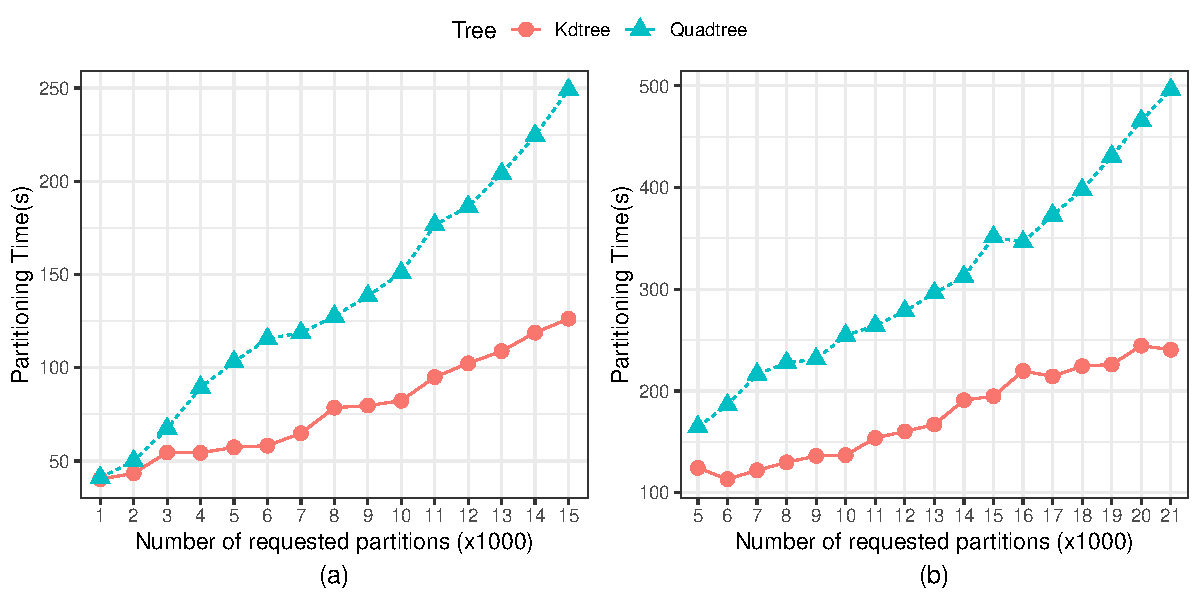
\includegraphics[width=\textwidth]{chapterExtension/K/K_Partitioning} 
    \caption{Data partitioning time using a spatial data structure (a) in the MainUS dataset and (b) in the GADM dataset.} \label{fig:k_partitioning_us}
 \end{figure}

 Figure \ref{fig:k_partitioning_us} presents the cost of partitioning the full content of both layers. Based on the sample tree data structure, each edge is assigned to a cell (partition) according to the leaf in which it is located; edges are assigned (or duplicated) to all leaves they intersect. A shuffle operation is then performed to move the data to the corresponding node responsible for handling each cell (partition). The figure shows that quadtree partitioning takes more time, primarily due to the larger number of leaves generated by the sample tree and the higher number of edges overlapping multiple partitions, which is expected with the quadtree’s use of smaller, more numerous cells.

\begin{figure}
    \centering
    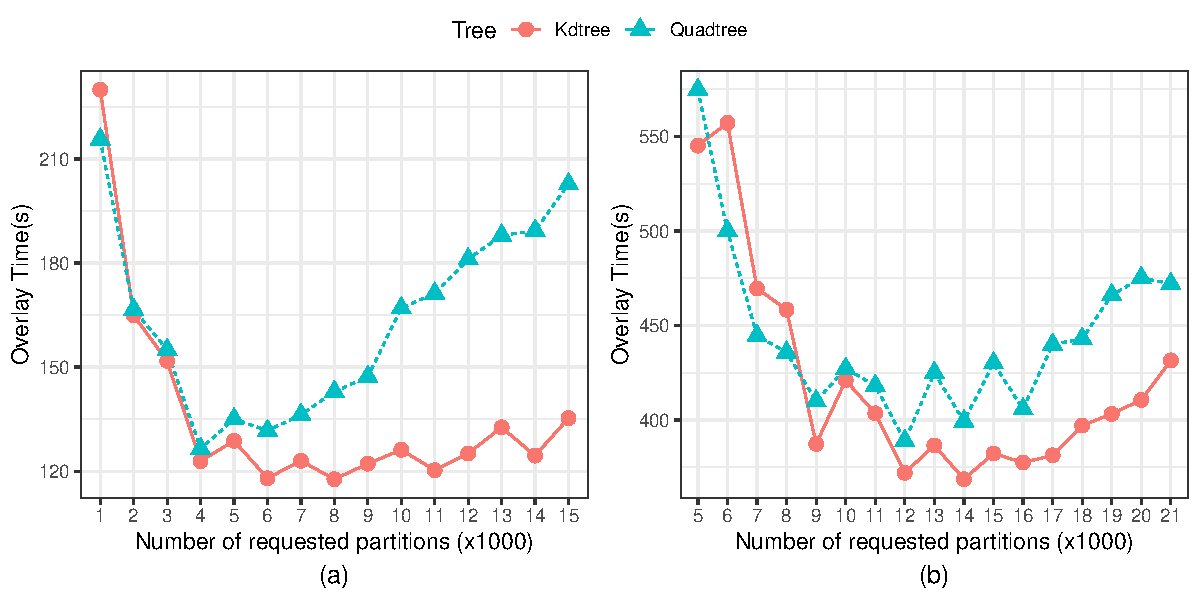
\includegraphics[width=\textwidth]{chapterExtension/K/K_Overlay} 
    \caption{Execution time for the overlay operation using a spatial data structure in the MainUS (a)and GADM (b) dataset.} \label{fig:k_overlay_us}
\end{figure}

Once the data is assigned to their respective partitions, the overlay operation can be executed.  Figure \ref{fig:k_overlay_us} illustrates the overlay performance for each partitioning strategy with varying numbers of cells. The kd-tree approach performs better, as the quadtree’s tendency to generate a higher number of empty cells negatively impacts its performance.

\begin{figure}
    \centering
    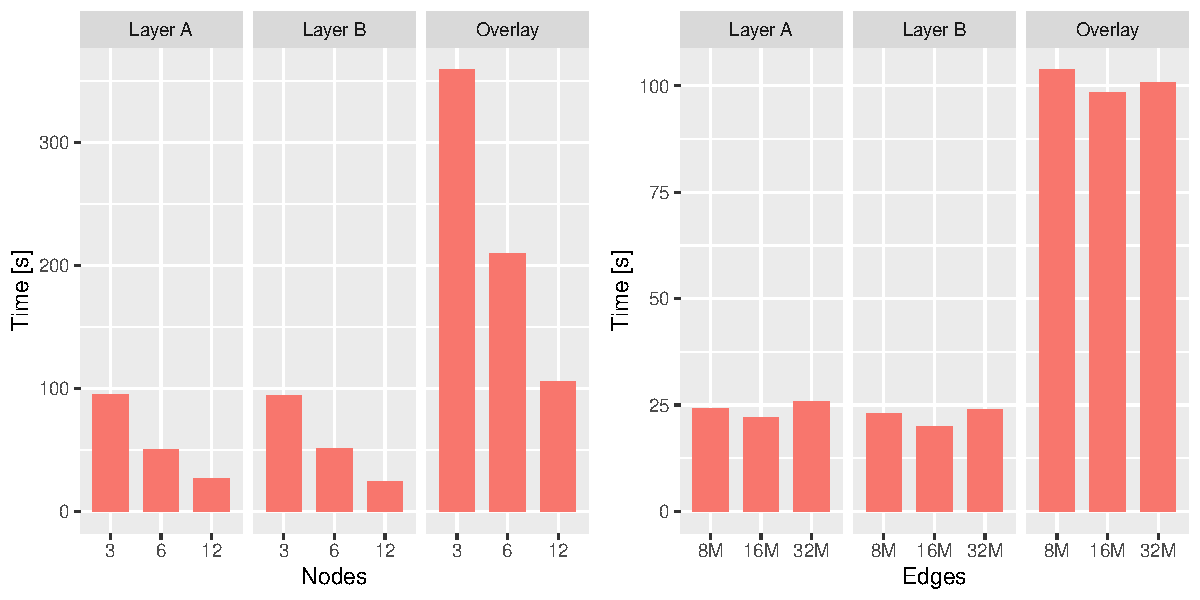
\includegraphics[width=\textwidth]{chapterExtension/K_SS/K_SS}
    \caption{(a)Speed Up and (b) Scale Up performance of the Kdtree partitioning using the MainUS dataset.} \label{fig:k_scale_speed_us}
\end{figure}

Finally, we evaluate the speed-up and scale-up performance of the kd-tree partitioning. Figure \ref{fig:k_scale_speed_us}(a) presents the speed-up performance for the MainUS dataset (36 million edges) as the number of nodes varies (3, 6, and 12 nodes). Similar to the quadtree partitioning strategy, the kd-tree partitioning demonstrates strong speed-up performance. Doubling the resources nearly halves the execution time, indicating effective scalability.

Figure \ref{fig:k_scale_speed_us}(b) illustrates the scale-up performance of the kd-tree partitioning approach. Following the procedure outlined in Section \ref{sec:speed_scale}, we generated datasets with 8M, 16M, and 32M edges from the MainUS dataset and applied the kd-tree partitioning strategy using 3, 6, and 12 nodes, respectively. The kd-tree partitioning demonstrates strong scale-up performance, maintaining consistent speed-up as the load per node remains nearly equal.

\subsection{Overlaying Polygons with Dangle and Cut Edges}

\begin{table}
    \small
    \caption{Overlaying Polygons with Dangle and Cut Edges Dataset}
    \label{tab:dangles}
    \begin{tabular}{c c c c}
        \toprule
        Dataset & Number Layer $A$ of Polygons & Number of Layer $B$ Edges & Result Polygons \\
        \midrule
        TN & 1,272 & 3,380,780 & 41,761 \\
        GA & 1,633 & 4,647,171 & 49,125 \\
        NC & 1,272 & 7,212,604 & 22,413 \\
        TX & 4,399  & 8,682,950 & 98,635 \\
        VA & 1,554 & 8,977,361 & 38,941 \\
        CA & 7,038 & 9,103,610 & 96,916\\
        \bottomrule
    \end{tabular}
\end{table}

\begin{figure}
    \centering
    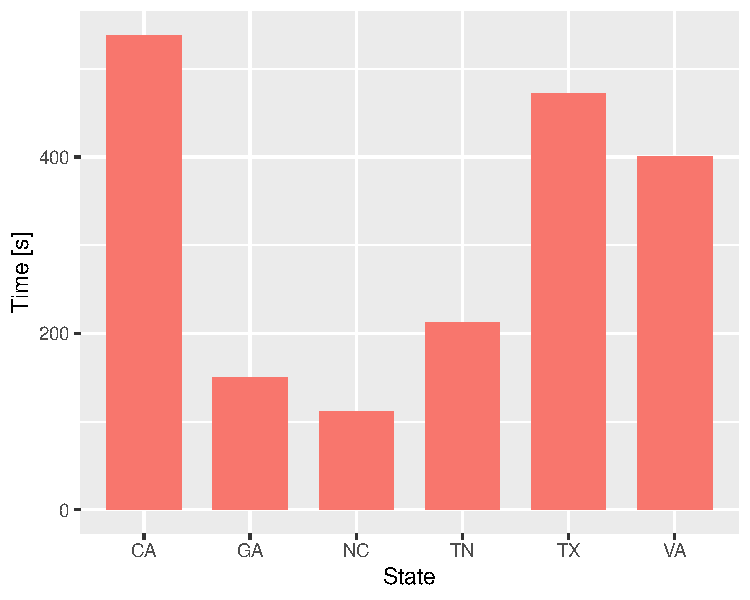
\includegraphics[width=0.6\textwidth]{chapterExtension/states.pdf}
    \caption{Overlaying State polygons with dangle and cut edges.}
    \label{fig:dangle}
\end{figure}

In this section, we examine the performance of overlaying polygons with dangle and cut edges resulting from the polygonization process, as detailed in \ref{sec:over_dang}.  Table \ref{tab:dangles} presents the number of polygons per state for the first overlay layer, the number of dangle and cut edges per state for the second overlay layer, and the number of resulting polygons per state.

From Figure \ref{fig:dangle}shows that the running time is influenced by both the number of dangle and cut edges and the number of intersections between the two layers (indicated by the number of generated polygons). TN and GA have relatively fewer dangle and cut edges, leading to lower execution times compared to VA, TX, and CA. However, because NC has significantly fewer intersections than TN and GA, it exhibits the lowest execution time overall. While TX, VA, and CA have a comparable number of edges, VA’s lower number of intersections results in a shorter execution time compared to TX and CA.
